\documentclass[12pt]{article}
\usepackage[margin=1in]{geometry}
\usepackage[utf8]{inputenc}
\usepackage[spanish]{babel}
\usepackage{parskip}
\usepackage{setspace}
\usepackage{amsmath}
\usepackage{graphicx}
\usepackage{tikz}
\usepackage{hyperref}

% Opciones de paquetes
\decimalpoint % {babel}: coma decimal como punto.
\onehalfspacing % {setspace}: interlineado
\graphicspath{{./img/}} % {graphicx}: Ruta (path) donde se encuentran las imagenes.
\usetikzlibrary{babel} % {tikz}: Para que tikz no conflictue con {babel} con figuras como "->".
\usetikzlibrary{arrows.meta} %{tikz}: Librería para personalizar las cabezas de las flechas.

% Encabezado.
\title{Clase 31. Longitud de Arco.}
\author{MIT 18.01: Single Variable Calculus.}
\date{}

\begin{document}

\maketitle

\begin{abstract}
\noindent La longitud de arco de una curva podemos conocerla mediante integrales. Veremos que al trabajar con ellas podemos obtener la noción precisa de esta medida, así como algunas fórmulas de figuras geométricas ya conocidas. Para ello, revisaremos ejemplos y calcularemos el área de la superficie de una figura en rotación.
\end{abstract}


\section{Longitud de Arco.}

En ocasiones estaremos interesados en conocer el \textbf{largo de la curva de una función entre dos puntos}. Si no es lineal en dicho lugar, quiere decir que estamos calculando la \textbf{longitud de arco}, la cual denotaremos como $s$.

\subsection{Fórmula de la longitud de arco.}

Supongamos que buscamos calcular la longitud de arco de una función $y = f(x)$ en el intervalo $a \leq x \leq b$, lugar en el cual es continua y derivable.

\begin{figure}[hbt!]
\centering

\begin{tikzpicture}
% help lines
%\draw[help lines] (-8, -1) grid (8, 4);

% Linea recta que une los puntos a y b, para ayudarnos en hacer la curva usando la curva cubica de Bezier.
%\draw [color = red] (-3, 0.1) -- (3, 2.9);

% Ejes.
\draw [-{Stealth[length=3mm, width=2mm]}] (-4.4, 0) -- (3.5, 0) node [below] {$x$};
\draw [-{Stealth[length=3mm, width=2mm]}] (-4, -0.4) -- (-4, 3.2) node [left] {$y$};

% Origen.
\node at (-4.2, -0.2) {$0$};

% Curva.
\draw [color = blue, line width = 0.3mm] (-3, 0.1) .. controls (-1.5, 3.5) and (1.4, -0.8) .. (3, 2.9);

% y = f(x)
\node at (3, 3.2) {$y = f(x)$};

% Lineas verticales.
\draw [dashed] (-2.7, 0) node [below] {$a$} -- (-2.7, 0.57);
\draw [dashed] (2.7, 0) node [below] {$b$} -- (2.7, 2.35);
\end{tikzpicture}

\end{figure}

Para lograr nuestro objetivo, lo primero que hacemos es dividir la curva de $f(x)$ mediante líneas verticales y luego, entre cada punto $P(x_{i}, \ y_{i})$, para $i = 1, \ 2, \ \cdots, \ n$, trazamos segmentos de rectas que forman una \textbf{trayectoria poligonal}.

\newpage

\begin{figure}[hbt!]
\centering

\begin{tikzpicture}
% help lines
%\draw[help lines] (-8, -1) grid (8, 4);
%\draw (0, -1) -- (0, 4);
%\draw (-8, 0) -- (8, 0);

% Linea recta que une los puntos a y b, para ayudarnos en hacer la curva usando la curva cubica de Bezier.
%\draw [color = red] (-3, 0.1) -- (3, 2.9);

% Ejes.
\draw [-{Stealth[length=3mm, width=2mm]}] (-4.4, 0) -- (3.5, 0) node [below] {$x$};
\draw [-{Stealth[length=3mm, width=2mm]}] (-4, -0.4) -- (-4, 3.2) node [left] {$y$};

% Origen.
\node at (-4.2, -0.2) {$0$};

% Curva.
\draw [color = blue, line width = 0.3mm] (-3, 0.1) .. controls (-1.5, 3.5) and (1.4, -0.8) .. (3, 2.9);

% y = f(x)
\node at (3, 3.2) {$y = f(x)$};

% Lineas verticales.
\draw [dashed] (-2.7, 0) node [below] {$a = x_{0}$} -- (-2.7, 0.65);
\draw [dashed] (2.7, 0) node [below] {$b = x_{n}$} -- (2.7, 2.3);
% Lineas verticales adicionales.
\draw [dashed] (-1.5, 0) node [below] {$x_{1}$} -- (-1.5, 1.5);
\draw [dashed] (0, 0) node [below] {$x_{i - 1}$} -- (0, 1.4);
\draw [dashed] (1.2, 0) node [below] {$x_{i}$} -- (1.2, 1.3);

% Trayectoria poligonal.
\draw [color = red] (-2.7, 0.65) -- (-1.5, 1.5) -- (0, 1.4) -- (1.2, 1.3) -- (2.7, 2.3);

% Puntos.
\draw [color = blue, fill = blue] (-2.7, 0.65) circle (0.6mm) node [left] {$P_{0}$};
\draw [color = blue, fill = blue] (-1.5, 1.5) circle (0.6mm) node [above] {$P_{1}$};
\draw [color = blue, fill = blue] (0, 1.4) circle (0.6mm) node [above] {$P_{i - 1}$};
\draw [color = blue, fill = blue] (1.2, 1.3) circle (0.6mm) node [above] {$P_{i}$};
\draw [color = blue, fill = blue] (2.7, 2.3) circle (0.6mm) node [right] {$P_{n}$};
\end{tikzpicture}

\end{figure}

La idea es \textbf{aproximarnos a la longitud de arco} de $f(x)$ mediante \textbf{el largo de la trayectoria poligonal}, que podemos obtener al sumar las medidas de cada segmento de recta $L_{i}$, las cuales, a su vez, es posible conocer por el teorema de Pitágoras. A continuación tenemos a una de ellas:

\begin{figure}[hbt!]
\centering

\begin{tikzpicture}
% Celdas de ayuda
%\draw [help lines] (-3, -3) grid (3, 3);

% Segmento trayectoria poligonal
\draw [color = red] (-2, 0) -- node [below] {$L_{i}$} (2, 2);

% Curva
\draw [color = blue, line width = 0.3mm] (-2, 0) .. controls (-1, 2) and (0, 2) .. node [above] {$\Delta s_{i}$}  (2, 2);

% Lineas verticales
\draw [dashed] (-2, -2) node [below] {$x_{i - 1}$} -- (-2, 0);
\draw [dashed] (2, -2) node [below] {$x_{i}$} -- (2, 2);

% Delta y_{i}.
\node at (2.4, 1) {$\Delta y_{i}$};

% Base triangulo rectangulo.
\draw[dashed] (-2, 0) -- node [below] {$\Delta x_{i}$} (2, 0);

% Angulo recto.
\draw (2, 0.3) -- (1.7, 0.3) -- (1.7, 0);

% Puntos
\draw [color = blue, fill = blue] (-2, 0) circle (0.6mm) node [left] {$P_{i - 1}$};
\draw [color = blue, fill = blue] (2, 2) circle (0.6mm) node [above] {$P_{i}$};
\end{tikzpicture}

\end{figure}

donde $\Delta s_{i}$ es la medida de una parte de la longitud de arco de $f(x)$ en $[a, \ b]$ y:
\[
  L_{i} = \sqrt{(\Delta x_{i})^{2} + (\Delta y_{i})^{2}}
\]
Nuestro propósito es aproximarnos a $\Delta s$ por medio de $L_{i}$. Es decir, que $\Delta s \approx L_{i}$.
\[
  \Delta s_{i} \approx \sqrt{(\Delta x_{i})^{2} + (\Delta y_{i})^{2}}
\]
Algo que suele hacerse en esta fórmula, es factorizar la raíz cuadrada por $(\Delta x)^{2}$.
\[
  \Delta s_{i} \approx \sqrt{1 + \left(\frac{\Delta y_{i}}{\Delta x_{i}}\right)^{2}} \cdot \Delta x_{i} 
\]
La razón $(\Delta y_{i} / \Delta x_{i})^{2}$ es la pendiente al cuadrado del segmento $L_{i}$. Debido a que $f(x)$ es continua y derivable en $[a, \ b]$, podemos garantizar por el \textbf{teorema del valor medio} que:

\[
  \frac{\Delta y_{i}}{\Delta x_{i}} = \left. \frac{dy_{i}}{dx_{i}} \right|_{x_{i} = c_{i}}, \ \text{ para } P_{i - 1} < c_{i} < P_{i}
\]
Hagamos el reemplazo en $\Delta s_{i}$.
\[
  \Delta s_{i} \approx \sqrt{1 + \left(\left. \frac{dy_{i}}{dx_{i}} \right|_{x_{i} = c_{i}}\right)^{2}} \cdot \Delta x_{i}
\]
En ese sentido, el largo de la trayectoria poligonal corresponde a:
\[
  \sum_{i = 1}^{n} \Delta s_{i} \approx \sum_{i = 1}^{n} \sqrt{1 + \left(\left. \frac{dy_{i}}{dx_{i}} \right|_{x_{i} = c_{i}}\right)^{2}} \cdot \Delta x_{i}
\]
Al dividir la curva de $f(x)$ en infinitas partes, el largo de la trayectoria poligonal irá igualándose a la longitud de arco de aquella función en $[a, \ b]$.
\[
\lim_{n \to \infty} \sum_{i = 1}^{n} \Delta s_{i} = 
  \lim_{n \to \infty} \sum_{i = 1}^{n} \sqrt{1 + \left(\left. \frac{dy_{i}}{dx_{i}} \right|_{x_{i} = c_{i}}\right)^{2}} \cdot \Delta x_{i}
\]
Es decir, la ecuación de arriba es equivalente a:
\[
  \int ds = \int_{a}^{b} \sqrt{1 + \left(\frac{dy}{dx}\right)^{2}} dx
\]
donde $\int ds$ es la \textbf{fórmula de la longitud de arco} de una función $y = f(x)$ en $[a, \ b]$.

Una forma más rápida de llegar a esta fórmula, es comenzar estableciendo que:
\[
  ds = \sqrt{dx^{2} + dy^{2}}
\]
Esto es válido porque, en lo infinitesimal, la suma de los diferenciales cuadráticos\footnote{Es bueno advertir que $dx^{2}$, $dy^{2}$ y $ds^{2}$ corresponden a $(dx)^{2}$, $(dy)^{2}$ y $(ds)^{2}$, respectivamente.} $dx^{2}$ y $dy^{2}$ serán iguales al correspondiente de la longitud de arco de la parte de la curva de $y = f(x)$, que es $ds^{2}$. Luego, $ds$ es simplemente la raíz cuadrada de dicha adición.

Posteriormente, factorizamos a $dx^{2}$ de la raíz cuadrada
\[
  ds = \sqrt{1 + \left(\frac{dy}{dx}\right)^{2}} dx
\]
y sumamos todos los diferenciales.
\[
  \int ds = \int_{a}^{b} \sqrt{1 + \left(\frac{dy}{dx}\right)^{2}} dx
\]
Otro aspecto a destacar es que
\[
  \int ds
\]
es una integral definida, no una indefinida. Generalmente trabajaremos con su fórmula y la que está expresada arriba es solo su notación matemática. No obstante, sus límites están definidos con respecto a la longitud de arco $s$ de $f(x)$, mientras que la de su ecuación es en términos de $x$ (o $y$, si estamos integrando en relación a aquella variable).

\subsection{Ejemplos del cálculo de la longitud de arco.}

\textbf{Ejemplo 1.} Calcule la longitud de arco de $y = mx$, con $m =$ constante, en el intervalo $0 \leq x \leq 10$.

\textbf{Solución.} Para usar la fórmula de la longitud de arco, debemos calcular la derivada de $y$, la cual es:
\[
  \frac{dy}{dx} = m
\]
Por lo tanto:
\[
  \int_{0}^{10} \sqrt{1 + m^{2}} dx = \sqrt{1 + m^{2}} \cdot \int_{0}^{10} 1 dx = 10 \sqrt{1 + m^{2}}
\]
La función $y = mx$ es, como sabemos, una función lineal. Si nos damos cuenta en este ejemplo, su longitud de arco entre $[0, \ 10]$ es igual a la hipotenusa de un triángulo rectángulo que podemos formar aquel intervalo.

\begin{figure}[hbt!]
\centering

\begin{tikzpicture}
%Lineas de ayuda.
%\draw[help lines] (-8, -1) grid (8, 3);

% Ejes.
\draw[->] (-5, 0) -- (2, 0) node [below] {$x$};
\draw[->] (-4, -0.5) -- (-4, 3) node [left] {$y$};

% Origen.
\node at (-4.2, -0.2) {$0$};

% Recta y = mx
\draw [color = blue, line width = 0.3mm] (-4.6, -0.3) -- (0.5, 2.3);

% Función.
\node at (0.5, 2.5) {$y = mx$};

% Recta vertical.
\draw [dashed] (0, 0) node [below] {$10$} -- (0, 2.05);

%Angulo recto.
\draw (0, 0.3) -- (-0.3, 0.3) -- (-0.3, 0);

% Medida de hipotenusa.
\node [rotate = 27] at (-2.4, 1.3) {$\sqrt{10^{2} + (10m)^{2}}$};

% Punto.
\draw [color = blue, fill = blue](0, 2.05) circle (0.6mm) node [right] {$(10, \ 10m)$};
\end{tikzpicture}

\end{figure}

donde $\sqrt{10^{2} + (10m)^{2}} = 10 \sqrt{1 + m^{2}}$.

Las conclusiones que podemos sacar de este ejemplo son:

\begin{enumerate}
\item La longitud de arco de una función lineal en un intervalo $[a, \ b]$ es igual a la hipotenusa de un triángulo rectángulo formado en dicho lugar.
\item La fórmula de la longitud de arco nos permite calcular aquella medida para funciones continuas lineales y no lineales.
\end{enumerate}

\textbf{Ejemplo 2.} Resuelva la longitud de arco $\alpha$ de $f(x) = \sqrt{1 - x^{2}}$ en el intervalo $[0, \ a]$.

\textbf{Solución.} En este caso estamos calculando la longitud de arco de un semicírculo unitario (i.e, de radio $r = 1$). Comencemos calculando la derivada de esta función.
\[
  \frac{d}{dx} f(x) = \frac{1}{2} (1 - x^{2})^{-1/2} (-2x) = - \frac{x}{\sqrt{1 - x^{2}}}
\]
Luego, calculemos $\alpha$ en $[0, \ a]$ de $f(x)$.
\[
  \alpha = \int_{0}^{a} \sqrt{1 + \left(- \frac{x}{\sqrt{1 - x^{2}}}\right)^{2}} dx
         = \int_{0}^{a} \frac{1}{\sqrt{1 - x^{2}}} dx
         = \left. \arcsin\left(\frac{x}{1}\right) \right|_{0}^{a}
         = \arcsin(a)
\]
En ese sentido, a partir de la longitud de arco que obtuvimos, también podemos señalar que:
\[
  \sin(\alpha) = a
\]
Lo cual es válido porque, como veremos a continuación, $\alpha$ está medido en radianes.

La longitud del arco de un círculo que subtiende a un ángulo $\theta$ en su centro, es una proporción de toda la circunferencia de esta figura, la cual es igual a la proporción de dicho ángulo con respecto al del círculo completo. Es decir, usando la notación de este ejemplo:
\[
  \frac{\alpha}{2 \pi r} = \frac{\theta}{\theta_{T}}; \ (\theta_{T} = \text{ángulo de todo el círculo})
\]
Como comúnmente $\theta$ se mide en \textbf{radianes} para calcular la longitud de arco de un círculo, entonces:
\begin{align*}
  \frac{\alpha}{2 \pi r} &= \frac{\theta}{2 \pi} \\
  \alpha &= \frac{\theta}{2 \pi} \cdot (2 \pi r) \\
  \alpha &= \theta r
\end{align*}
En este ejemplo trabajamos con un semicírculo unitario, por tanto
\[
  \alpha = \theta
\]
Ahora, tenemos que comprobar que el $\sin(\alpha) = a$. Veámoslo a nivel geométrico.

\begin{figure}[hbt!]
\centering

\begin{tikzpicture}
% Lineas de ayuda.
%\draw [help lines] (-8, -1) grid (8, 3.5);

% Ejes.
\draw [<->] (-4, 0) -- (4, 0) node [below] {$x$};
\draw [->] (0, -0.5) -- (0, 3.3) node [left] {$f(x)$};

% Origen
\node at (-0.2, -0.25) {$0$};

% Semi circulo.
\draw (3, 0) node [below] {$1$} arc [start angle = 0, end angle = 180, x radius = 3, y radius = 3];

% Línea vertical y horizontal segmentada.
\draw [dashed] (2, 0) node [below] {$a$} -- (2, 2.23) -- node [above] {$a$} (-0.05, 2.23);

% Arco.
%\draw [color = red] (2, 2.23) -- (0, 3);
\draw [color = blue, line width = 0.45mm] (2, 2.23) .. controls (1.25, 2.7) and (1.4, 2.78) .. (0, 3);
\node [color = blue] at (1.5, 2.9) {$\alpha$};

% Rayo de \theta.
\draw (0, 0) -- (2, 2.23);
\node at (0.3, 0.7) {$\theta$};

% Medida de hipotenusa.
\node [rotate = 43] at (1.15, 0.85) {$1$};

% Ángulo recto.
\draw (0, 2) -- (0.25, 2) -- (0.25, 2.23);
\end{tikzpicture}

\end{figure}

Como se puede apreciar:
\[
  \sin(\theta) = \sin(\alpha) = \frac{a}{1} = a
\]
Y, por consiguiente:
\[
  \alpha = \arcsin(a)
\]
A partir de este ejemplo hemos encontrado una forma más rigurosa de calcular la longitud de arco de un círculo por medio de una integral. Además, esto nos permitió conocer del mismo modo al $\arcsin(x)$ y $\sin(x)$, lo cual también se aplica con las demás funciones trigonométricas. Es decir, obtuvimos una herramienta para conocer la procedencia de estas fórmulas.

\textbf{Ejemplo 3.} Calcule la longitud de arco de $f(x) = x^{2}$ en $[0, \ a]$.

\textbf{Solución.} Este ejemplo nos muestra aún más la utilidad de la fórmula de la longitud de arco que hemos visto, puesto que si bien en los anteriores podíamos resolverlos sin necesariamente usar el Cálculo\footnote{Por decirlo de algún modo, ya tenemos fórmulas ``pre-fabricadas'' para calcular la longitud de arco de una recta o un círculo.}, acá sí es necesario.

Debido a que la derivada de $f(x)$ es
\[
  \frac{d}{dx} f(x) = 2x,
\]
su longitud de arco $s$ en $[0, \ a]$ se define como:
\[
  s = \int_{0}^{a} \sqrt{1 + (2x)^{2}} dx = \int_{0}^{a} \sqrt{1 + 4x^{2}} dx
\]
En estricto rigor, podemos dar por resuelto la longitud de arco de $f(x) = x^{2}$ a partir de la integral que acabamos de obtener. Dependerá de nosotros si la evaluamos o no, sea de forma analítica o numérica. En este caso continuaremos, pero se debe advertir que su cálculo será largo.

Por la forma del integrando de $s$, la mejor opción es realizar una sustitución trigonométrica. En particular, como su expresión es del tipo $\sqrt{a + x^{2}}$ conviene establecer que:
\[
  x = \frac{1}{2} \tan(u) \quad \text{y} \quad dx = \frac{1}{2} \sec^{2}(u) du,
\]
implicando, primero, que:
\[
  \sqrt{1 + 4x} = \sqrt{1 + 4 \left(\frac{1}{2} \tan(u)\right)^{2}}
                = \sqrt{1 + \tan^{2}(u)}
                = \sqrt{\sec^{2}(u)}
                = \sec(u)
\]
y, en segundo lugar, que los limites de la integral son
\begin{align*}
  a &= \frac{1}{2} \tan(u) & 0 &= \frac{1}{2} \tan(u) \\
  2a &= \tan(u)            & 0 &= \tan(u) \\
  u &= \arctan(2a) & u     &= \arctan(0) = 0
\end{align*}
Por consiguiente:
\[
  s = \int_{0}^{a} \sqrt{1 + 4x^{2}}dx
    = \int_{0}^{\arctan(2a)} \frac{1}{2} \left(\sec(u) \cdot \sec^{2}(u)\right) du
    = \frac{1}{2} \int_{0}^{\arctan(2a)} \sec(u)^{3} du
\]
Continuemos con la integral trigonométrica sin la constante $(1/2)$ ni sus límites para buscar de forma más ordenada su antiderivada.
\[
  \int \sec^{3}(u) du
\]
Como probablemente lo notamos, es posible escribir esta integral como:
\[
  \int \sec^{3}(u) du = \int \sec^{2}(u) \sec(u) du
\]
De este modo, podemos resolverla usando la técnica de integración por partes, donde
\[
  v = \sec(u) \quad \text{y} \quad dw = \sec^{2}(u),
\]
lo que significa que:
\[
  dv = \sec(u) \tan(u) \quad \text{y} \quad w = \tan(u)
\]
En consecuencia:
\begin{align*}
  \int \sec^{3}(u) du &= \sec(u) \tan(u) - \int \tan(u) (\sec(u) \tan(u)) du \\
                      &= \sec(u) \tan(u) - \int \sec(u) \tan^{2}(u) du
\end{align*}
Puesto que $\sec^{2}(u) = 1 + \tan^{2}(u)$, entonces
\[
  \tan^{2}(u) = \sec^{2}(u) - 1
\]
Reemplazando en la integral de arriba obtenemos que:
\begin{align*}
  \int \sec^{3}(u) du &= \sec(u) \tan(u) - \int \sec(u) (\sec^{2} - 1) du \\
                      &= \sec(u) \tan(u) - \int \left(\sec^{3}(u) - \sec(u)\right) du \\
  \int \sec^{3}(u) du &= \sec(u) \tan(u) - \int \sec^{3}(u) du + \int \sec(u) du
\end{align*}
Cuando en la integración por partes uno de los términos se repite en ambos lados de la ecuación, quiere decir que estamos en frente de una fórmula recursiva o de reducción. Por ahora continuemos resolviéndola, sumando a la igualdad por $+ \int \sec^{3}(u)du$.
\begin{align*}
  2 \int \sec^{3}(u) du &= \sec(u) \tan(u) + \int \sec(u)du \\
  \int \sec^{3}(u) du &= \frac{1}{2} \left(\sec(u) \tan(u) + \int \sec(u)du\right)
\end{align*}
En la Clase 28 vimos que:
\[
  \int \sec(x)dx = \ln(|\sec(x) + \tan(x)|) + C
\]
Por lo tanto:
\[
  \int \sec^{3}(u) du = \frac{1}{2} \left(\sec(u) \tan(u) + \ln(|\sec(u) + \tan(u)|)\right)
\]
Ahora volvamos a la integral definida junto con la constante $(1/2)$.
\begin{align*}
  \frac{1}{2} \int_{0}^{\arctan(2a)} \sec^{3}(u) du &= \frac{1}{2}\left(\frac{1}{2}[\sec(u) \tan(u) + \ln(|\sec(u) + \tan(u)|)]_{0}^{\arctan(2a)}\right) \\
                                                    &= \frac{1}{4} \left[\sec(u) \tan(u) + \ln(|\sec(u) + \tan(u)|)\right]_{0}^{\arctan(2a)}
\end{align*}
Hasta ahora la integral está evaluada, pero tratemos de restituir a la variable $x$. Para ello, primero usemos otra vez la identidad trigonométrica:
\[
  \sec^{2}(u) = \tan^{2}(u) + 1
\]
En particular, utilicemos la raíz cuadrada de esta identidad para obtener a la $\sec(u)$.
\[
  \sec(u) = \sqrt{\tan^{2}(u) + 1}
\]
Reemplacemos a la $\sec(u)$ en la integral definida.
\begin{align*}
  &\frac{1}{2} \int_{0}^{\arctan(2a)} \sec^{3}(u) du = \\
  &\frac{1}{4} \left[
                 \left(\sqrt{\tan^{2}(u) + 1}\cdot \tan(u) \right) +
                 \ln\left(\left|\sqrt{\tan^{2}(u) + 1} + \tan(u)\right|\right)
               \right]_{0}^{\arctan(2a)}
\end{align*}
Luego, recordemos que:
\[
  x = \frac{1}{2} \tan(u)
\]
Despejemos a $\tan(u)$ de esta igualdad.
\[
  2x = \tan(u)
\]
Por otra parte, regresemos al límite superior de la integral en términos de $x$.
\[
  u = \arctan(2a) \Rightarrow \tan(u) = 2a \Rightarrow \frac{1}{2} \tan(u) = a
\]
De este modo, al reemplazar a la $\tan(u)$ por la expresión $2x$ en la integral y a sus límites, obtenemos que:

\begin{align*}
  \frac{1}{2} \int_{0}^{\arctan(2a)} \sec^{3}(u) du &= \frac{1}{4}
                                                       \left[
                                                         \left(\sqrt{1 + (2x)^{2}} \cdot 2x \right) +
                                                         \ln\left(\left|\sqrt{1 + (2x)^{2}} + 2x \right|\right)
                                                       \right]_{0}^{a} \\
                                                    &= \frac{1}{4}
                                                       \left[
                                                         2x \sqrt{1 + 4x^{2}} +
                                                         \ln\left(\left|\sqrt{1 + 4x^{2}} + 2x \right|\right)
                                                       \right]_{0}^{a} \\
  \frac{1}{2} \int_{0}^{\arctan(2a)} \sec^{3}(u) du &= \left[
                                                         \frac{1}{2} x \sqrt{1 + 4x^{2}} + 
                                                         \frac{1}{4} \ln\left(\left|\sqrt{1 + 4x^{2}} + 2x \right|\right)
                                                       \right]_{0}^{a}
\end{align*}
En otras palabras, la longitud de arco de $f(x) = x^{2}$ en $[0, \ a]$ es:
\[
  s = \int_{0}^{a} \sqrt{1 + 4x^{2}} dx = \left[
                                            \frac{1}{2} x \sqrt{1 + 4x^{2}} + 
                                            \frac{1}{4} \ln\left(\left|\sqrt{1 + 4x^{2}} + 2x \right|\right)
                                          \right]_{0}^{a}
\]
Antes de terminar este ejemplo, escribamos la \textbf{fórmula de reducción de la $\sec(x)$} para tenerla a mano junto con las que conocimos en la clase anterior.
\[
  \int \sec^{n}(x) dx = \frac{\sec^{n - 2}(x) \tan(x)}{n - 1} + \frac{n - 2}{n - 1} \int \sec^{n - 2}(x) dx \quad (\text{para } n \neq 1)
\]


\section{Aplicación: Áreas de Superficies.}

A partir de la \textbf{fórmula de la longitud de arco} podemos obtener otra ecuación para calcular el \textbf{área de una superficie} generada por una figura plana en rotación. La lógica es similar al cálculo del volumen de un sólido de revolución (Clase 22).

Sea $y = f(x) \geq 0$ una función continua y derivable. Supongamos que la hacemos girar con respecto al eje $x$ en el intervalo $[a, \ b]$.

\begin{figure}[hbt!]
\centering
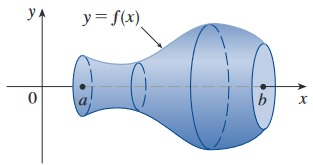
\includegraphics[scale=0.7]{surface-area-1.jpg}
\caption{Steward (2017). \textit{Cálculo. Trascendentes Tempranas}. Pp 552.}
\end{figure}

Para conocer el área de su superficie, cortamos una parte de ella en $[x_{i - 1}, \ x_{i}] \in [a, \ b]$ y demarcamos los puntos $P_{i - 1}(x_{i - 1}, \ y_{i - 1})$ y $P_{i}(x_{i}, \ y_{i})$, los cuales unimos mediante un segmento de recta de medida $L_{i}$.

\newpage

\begin{figure}[hbt!]
\centering
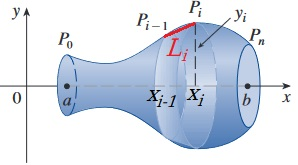
\includegraphics[scale=0.7]{surface-area-2.jpg}
\caption{Steward (2017). \textit{Cálculo. Trascendentes Tempranas}. Pp 552 (con arreglos propios).}
\end{figure}

La figura que se forma en la superficie de $f(x)$ es el \textbf{tronco de un cono} (i.e, sin su punta), por tanto su área se calcula como el producto entre la circunferencia de ambas caras de la sección transversal y el largo de su altura inclinada $L_{i}$.
\[
  A_{i} = (2 \pi r) \cdot L_{i}
\]
donde $r$ es el \textbf{radio promedio}\footnote{En los textos \textit{Cálculo. Trascendentes Tempranas} (Stewart, 2017: 551-552.) y \textit{Calculus With Analytic Geometry} (Simmons, 1996: 240-241) se explica con más detalle cómo se obtiene este radio.} calculado a partir del radio superior $r_{i} = y_{i}$ y el inferior $r_{i - 1} = y_{i - 1}$ de las dos secciones transversales.
\[
  r = \frac{y_{i - 1} + y_{i}}{2}
\]
Por otra parte, $L_{i}$ sabemos que corresponde a la hipotenusa del triángulo rectángulo que es posible formar con este segmento de recta.
\[
  L_{i} = \sqrt{(\Delta x_{i})^{2} + (\Delta y_{i})^{2}}
        = \sqrt{1 + \left(\frac{\Delta y_{i}}{\Delta x_{i}}\right)^{2}} \cdot \Delta x_{i}
        = \sqrt{1 + \left(\left. \frac{dy_{i}}{dx_{i}} \right|_{x_{i} = c_{i}}\right)^{2}} \Delta x_{i}
\]
donde $P_{i - 1} < c_{i} < P_{i}$.

Es decir:
\begin{align*}
  A_{i} = 2 \pi \cdot \left(\frac{y_{i - 1} + y_{i}}{2}\right) \cdot
           \sqrt{1 + \left(\left. \frac{dy_{i}}{dx_{i}} \right|_{x_{i} = c_{i}}\right)^{2}} \Delta x_{i}
        = \pi \cdot (y_{i - 1} + y_{i}) \cdot
           \sqrt{1 + \left(\left. \frac{dy_{i}}{dx_{i}} \right|_{x_{i} = c_{i}}\right)^{2}} \Delta x_{i}
\end{align*}
Por lo tanto, el área de superficie $A$ de $y = f(x)$ en $[a, \ b]$ se aproxima a la suma de las áreas $A_{i}$, con $i = 1, \ 2, \ \cdots \ n$, de los troncos de cono.

\[
  A \approx \sum_{i = 1}^{n} A_{i}
    = \sum_{i = 1}^{n} \pi \cdot (y_{i - 1} + y_{i}) \cdot \sqrt{1 + \left(\left. \frac{dy_{i}}{dx_{i}} \right|_{x_{i} = c_{i}}\right)^{2}} \Delta x_{i}
\]
Para tener una mejor aproximación al área, aumentamos las divisiones del área de la superficie de $y = f(x)$. En otras palabras,
\[
  A = \lim_{n \to \infty} \sum_{i = 1}^{n} A_{i}
    = \lim_{n \to \infty} \sum_{i = 1}^{n} \pi \cdot (y_{i - 1} + y_{i}) \cdot
      \sqrt{1 + \left(\left. \frac{dy_{i}}{dx_{i}} \right|_{x_{i} = c_{i}}\right)^{2}} \Delta x_{i}
\]
A medida que $n \to \infty$, la distancia $|x_{i} - x_{i - 1}| \to 0$. Por lo tanto, eventualmente $y_{i - 1} = y_{i}$. Esto significa que:
\[
  y_{i - 1} + y_{i} = 2y_{i}, \ \text{ cuando } n \to \infty
\]
En consecuencia:
\[
  A = \lim_{n \to \infty} \sum_{i = 1}^{n} A_{i}
    = \lim_{n \to \infty} \sum_{i = 1}^{n} 2 \pi y_{i} \cdot \sqrt{1 + \left(\left. \frac{dy_{i}}{dx_{i}} \right|_{x_{i} = c_{i}}\right)^{2}} \Delta x_{i}
\]
Lo que es equivalente a:
\[
  A = \int_{a}^{b} dA
    = \int_{a}^{b} 2 \pi y \cdot \sqrt{1 + \left(\frac{dy}{dx}\right)^{2}} dx
    = \int_{a}^{b} 2 \pi y \cdot ds
\]
que corresponde al \textbf{área de superficie de $y = f(x)$ en $[a, \ b]$}, mientras que $ds$ es la longitud de arco de la misma función y en el mismo intervalo.

\textbf{Ejemplo 4.} Calcule el área de la superficie generada por $f(x) = x^{2}$ al ser rotada alrededor del eje $x$ en $[0, \ a]$.

\textbf{Solución.} Usemos la fórmula para calcular áreas de superficies, donde ya sabemos por el ejemplo anterior que la longitud de arco de $f(x) = x^{2}$ expresada como integrando es $\sqrt{1 + 4x^{2}}$.
\[
  A = \int_{0}^{a} 2 \pi \cdot x^{2} \sqrt{1 + 4x^{2}} dx
\]
En esta ocasión no resolveremos esta integral, pero usando sustitución trigonométrica estableciendo que $x = (1/2) \tan(u)$ y, luego, con la fórmula de reducción de la $\sec^{n}(u)$ vista anteriormente, obtenemos que:
\[
  A = \frac{\pi}{32} \left[4x (4x^{2} + 1)^{3/2} - 2x \sqrt{4x^{2} + 1} - \ln\left(\left|2x + \sqrt{4x^{2} + 1} \right|\right) \right]_{0}^{a}
\]

\textbf{Ejemplo 5.} Calcule el área de superficie de una esfera de radio $r = a$ generada por el semicírculo $f(x) = \sqrt{a^{2} - x^{2}}$ al ser girada con respecto a $x$ en el intervalo $[x_{1}, \ x_{2}]$.

\textbf{Solución.} El integrando de $f(x)$ lo vimos en el Ejemplo 2, donde en dicho caso correspondió a un semicírculo unitario. Acá es de $r = a$, por lo que obtendremos que
\[
  ds = \sqrt{\frac{a^{2}}{a^{2} - x^{2}}} = \frac{a}{\sqrt{a^{2} - x^{2}}}
\]
Así:
\begin{align*}
  A = \int_{x_{1}}^{x_{2}} 2 \pi \left(\sqrt{a^{2} - x^{2}}\right) \cdot \frac{a}{\sqrt{a^{2} - x^{2}}} dx
    = 2 \pi a \int_{x_{1}}^{x_{2}} 1 dx 
    = (2 \pi a) \cdot (x_{2} - x_{1})
\end{align*}
Cuando obtenemos fórmulas sencillas al evaluar la integral como lo fue en este caso, siempre es bueno probarla estableciendo valores arbitrarios en los límites. Por ejemplo, veamos el área de superficie para toda la esfera. Es decir, para $x_{1} = -a$ y $x_{2} = a$.
\[
  A = (2 \pi a) \cdot (a - (-a)) = (2 \pi a) \cdot 2a = 4 \pi a^{2}
\]
Cuya expresión corresponde al área de superficie de toda una esfera de radio $r = a$.
\end{document}
